\documentclass[a4paper]{report}
\usepackage[english]{babel}
\usepackage{amssymb}
\usepackage{amsmath}
\usepackage{graphicx}
\usepackage{float}
\usepackage{shortvrb}
\usepackage{cancel}
\usepackage[T1]{fontenc}
\usepackage{hyperref}
\usepackage{epstopdf}
%Makes it possible to ignore other preambles of child document
\usepackage{standalone}

%Possible to change the margins
\usepackage{geometry}
\geometry{verbose,tmargin=1.9cm,bmargin=1.7cm,lmargin=1cm,rmargin=1cm}

\usepackage{subfig}

%include pdf pages
\usepackage{pdfpages}

%being able to create tables over multiple pages
\usepackage{longtable}

\makeatletter

%Change standard font size
\renewcommand\normalsize{ \@setfontsize\normalsize{11pt}{11pt}}\normalsize  

\makeatother

\usepackage{fancyhdr}
\pagestyle{fancy}
\fancyhead{}
\fancyfoot{}

%Gives text above each page
\fancyhead[CO,CE]{DSE Project}

%Page number
\fancyfoot[RO,LE]{\thepage}

\usepackage{babel}

%Available structures:
%Report: \part{}, \chapter{}, \section{}, \subsection{}, \subsubsection{}, \paragraph{}, \subparagraph{}

\begin{document}
\chapter{Schedule and Work Logic}
This chapter will document the planning at its current state for the entire project. The schedule is developed with the rolling wave principle in mind. Therefore the schedule below is presented in a detailed level up to the midterm report deadline and the schedule after that is only broadly planned. In order to be able to make a detailed planning, the project work-flow logic has to be considered simultaneously. Thus the work-flow logic will also be discussed in this chapter and the results will be presented in a Work-Flow Diagram (WFD). 

First the project milestones will be discussed, after which the project phasing will be presented. Since the phasing is also dependent on the work-flow logic, this will be discussed alongside it. The graphical results of these discussions will be presented in the form of a Gantt chart and Work-Flow Diagrams. Finally, the Work Breakdown Structure (WBS) diagram will also be shown, which is derived from the Gantt chart logic. Once the schedule has been discussed, some time will be spent to locate the scheduling risks.
\section{Milestones}
Three milestone reviews have been set. A Baseline Review (BR) is planned for May 6$^{th}$, a Midterm Review (MTR) is planned for May 30$^{th}$ and  the Final Review (FR) is planned for June 27$^{th}$. An additional milestone can be set for the DSE Symposium Day for July 4$^{th}$, at which point the results of the final Final Review have to be presented to a jury of experts. \newline

The deliverables for the Baseline Review are a Project Plan (PP) and the Baseline Report. The deliverables for the Midterm Review are a Midterm Report and the presentation of the results. For the Final Review the deliverables are the Final Report and a presentation on the results. Finally, for the Symposium a presentation and a poster need to be delivered. \newline

When developing the schedule, in general the deadlines for the milestones were used. The only exception is the Project Plan, which is due to be delivered on May 6$^{th}$. Internally the group has set a deadline for the Project Plan on April 26$^{th}$, in order to focus all the resources afterwards on the Baseline Report. 

\section{Project Phasing and Logic}
Now the milestones and deadlines are known, these can be used as a fixture to build the schedule around. The scheduling for each milestone will now be treated separately below. The Project Plan will be included with the Baseline Review milestone. 
\subsection{Baseline Review}
The first part of the Baseline Review concerns the Project Plan. Various tasks were defined in accordance to the deliverables listed in the Project Plan requirements. The task for Work Break-Down (WBS) structure was subdivided into the various specialty groups as defined in chapter \ref{Chapter:Teamorganization}. These specialty groups defined a more detailed work breakdown schedule once the general WBS was developed. Obviously the assignment of the human resources was dependent on the group organization, thus every task had to wait before this was completed. Once that was done, the work on the WBS, the Gantt chart and the Work-Flow Diagrams (WFD) could proceed in parallel. Finally, when this work was divided some spare human resources remained. These were assigned to perform the market analysis. \newline
\noindent
The Gantt chart for the Project Plan and Baseline Review can be seen in \autoref{fig:ganttbr}. This figure shows the critical tasks of the Project Plan are the Gantt chart and the WFD.
\begin{figure}[h]
	\centering
	
	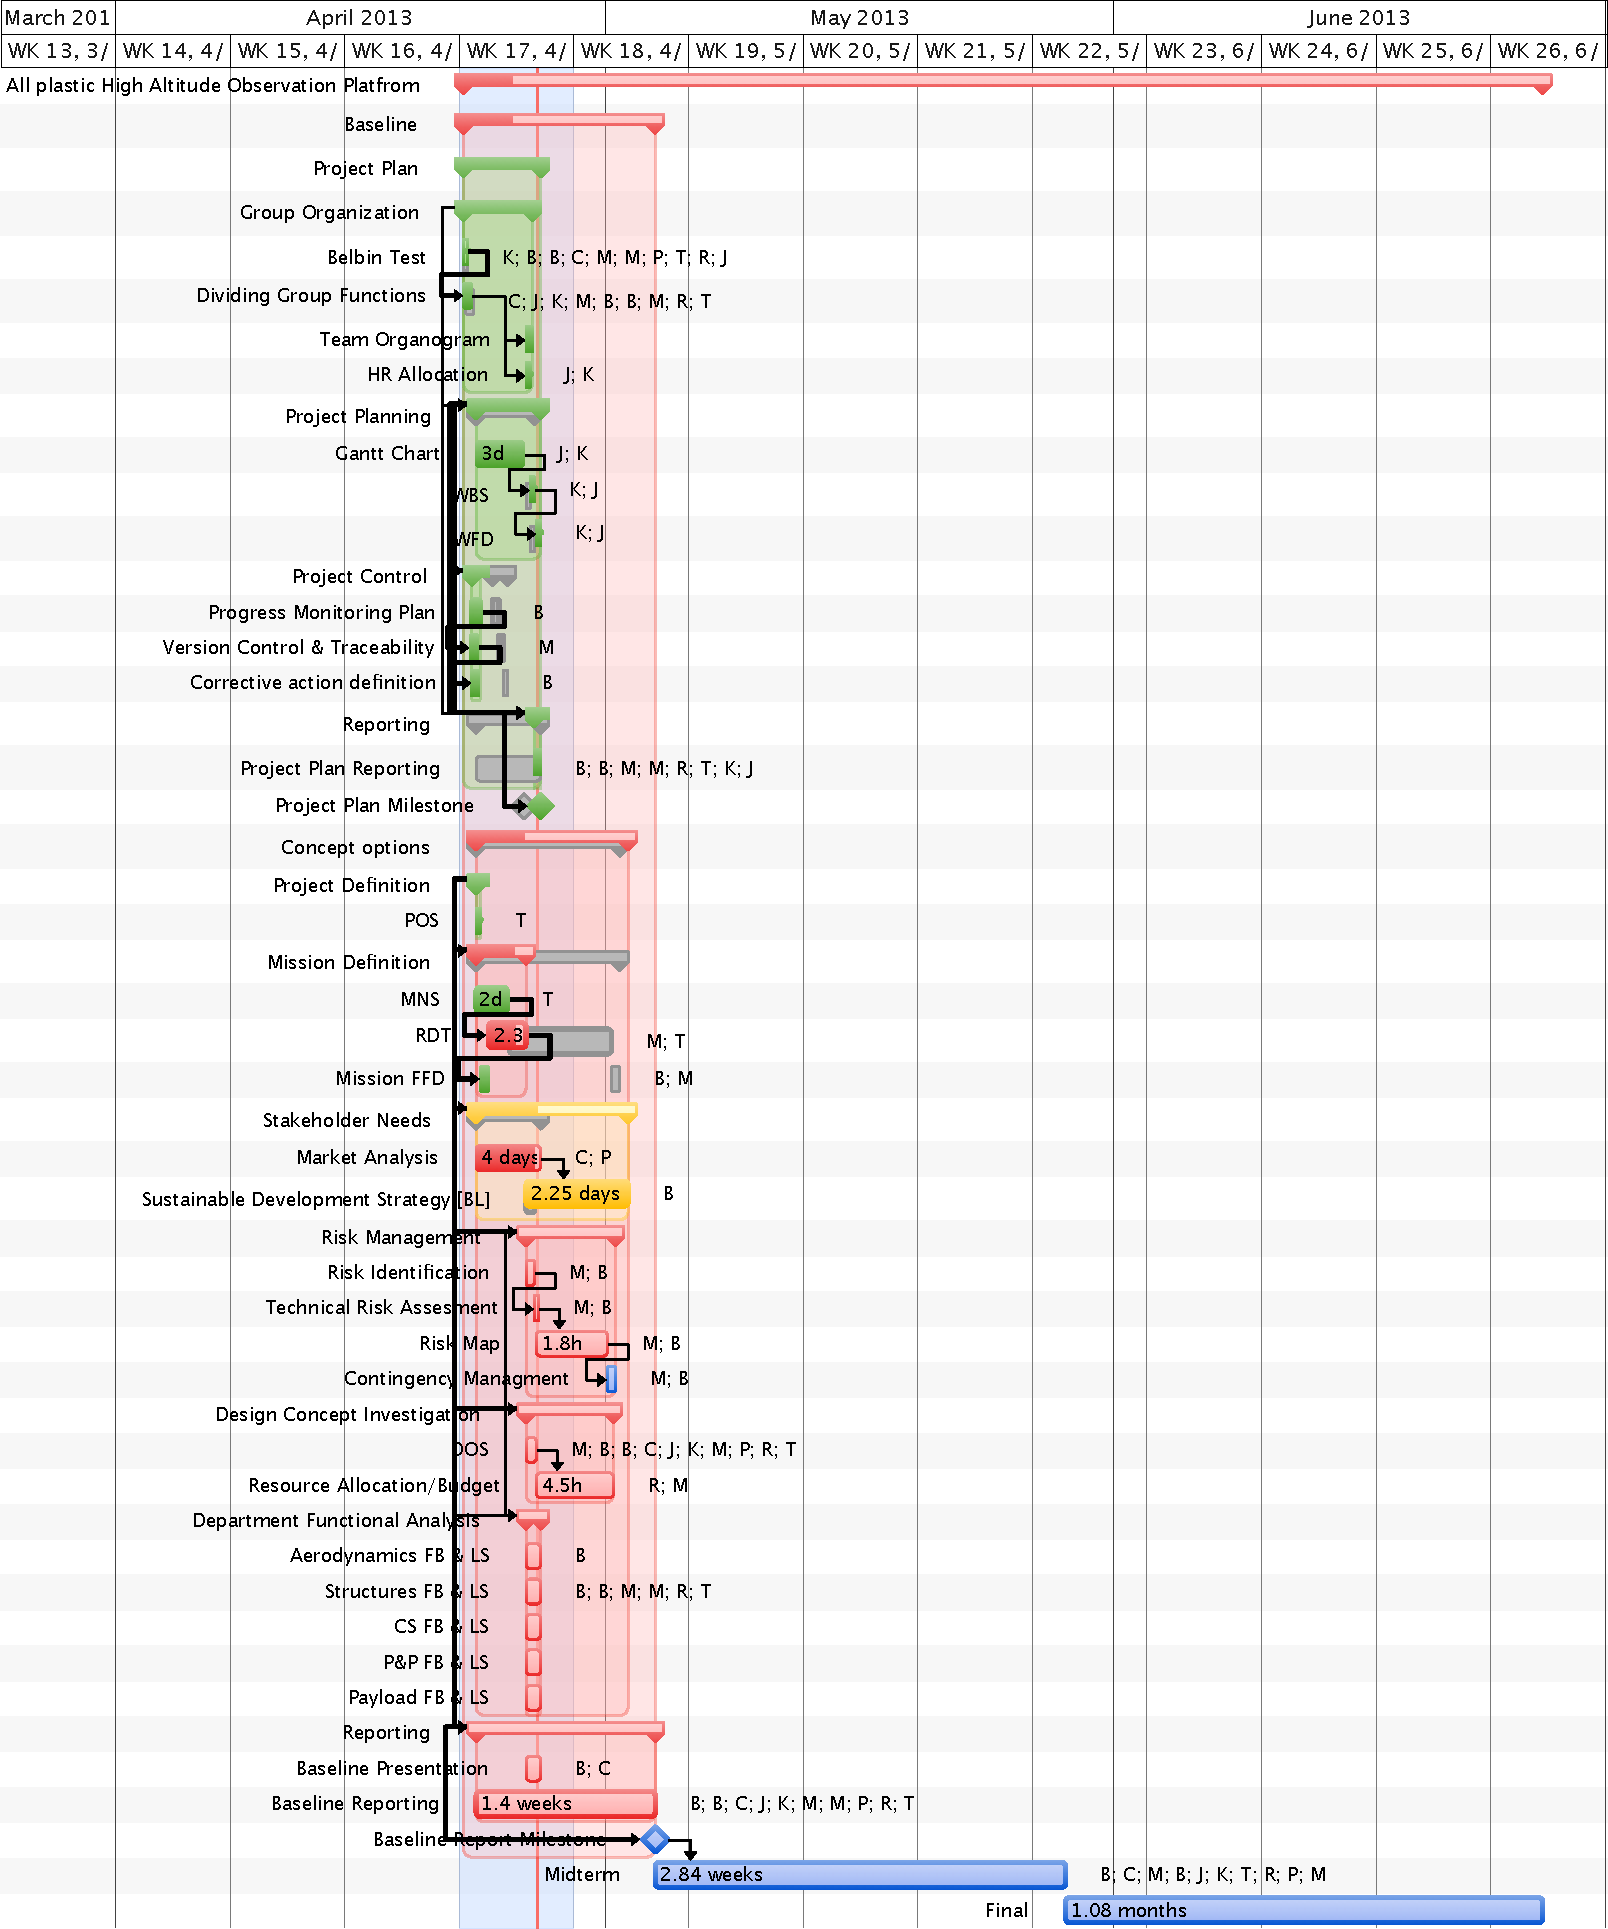
\includegraphics[width=0.7\textwidth]{Figures/BASEGANTT.PDF}
	\caption{Gantt chart of the PP and BR schedule}
	\label{fig:ganttbr}
	
\end{figure}
The logical structure of the Gantt chart can be seen in \autoref{fig:wfdbr}. It can clearly be seen many of the tasks can be performed in parallel of each other. 

\subsection{Baseline Report}
\autoref{fig:ganttbr} also shows the Gantt chart for the Baseline Report planning. Apart from the deliverables specified, an extra task was added to the chart. A day is reserved for a literature study, to allow each specialist group to gain knowledge about the theory and the state of the art technology concerning their field. \newline
\noindent
There are several dependencies between the various tasks, which means work needs to proceed in a more sequential fashion. Sustainable development strategy is linked to market analysis because sustainable development is becoming more and more a market driven requirement. The Requirement Discovery Tree needs to be  developed before a Design Option Structuring tree (DOS) can be made. The logic can be seen in \autoref{fig:wfdbr}.
\begin{figure}[H]
	\centering
	
	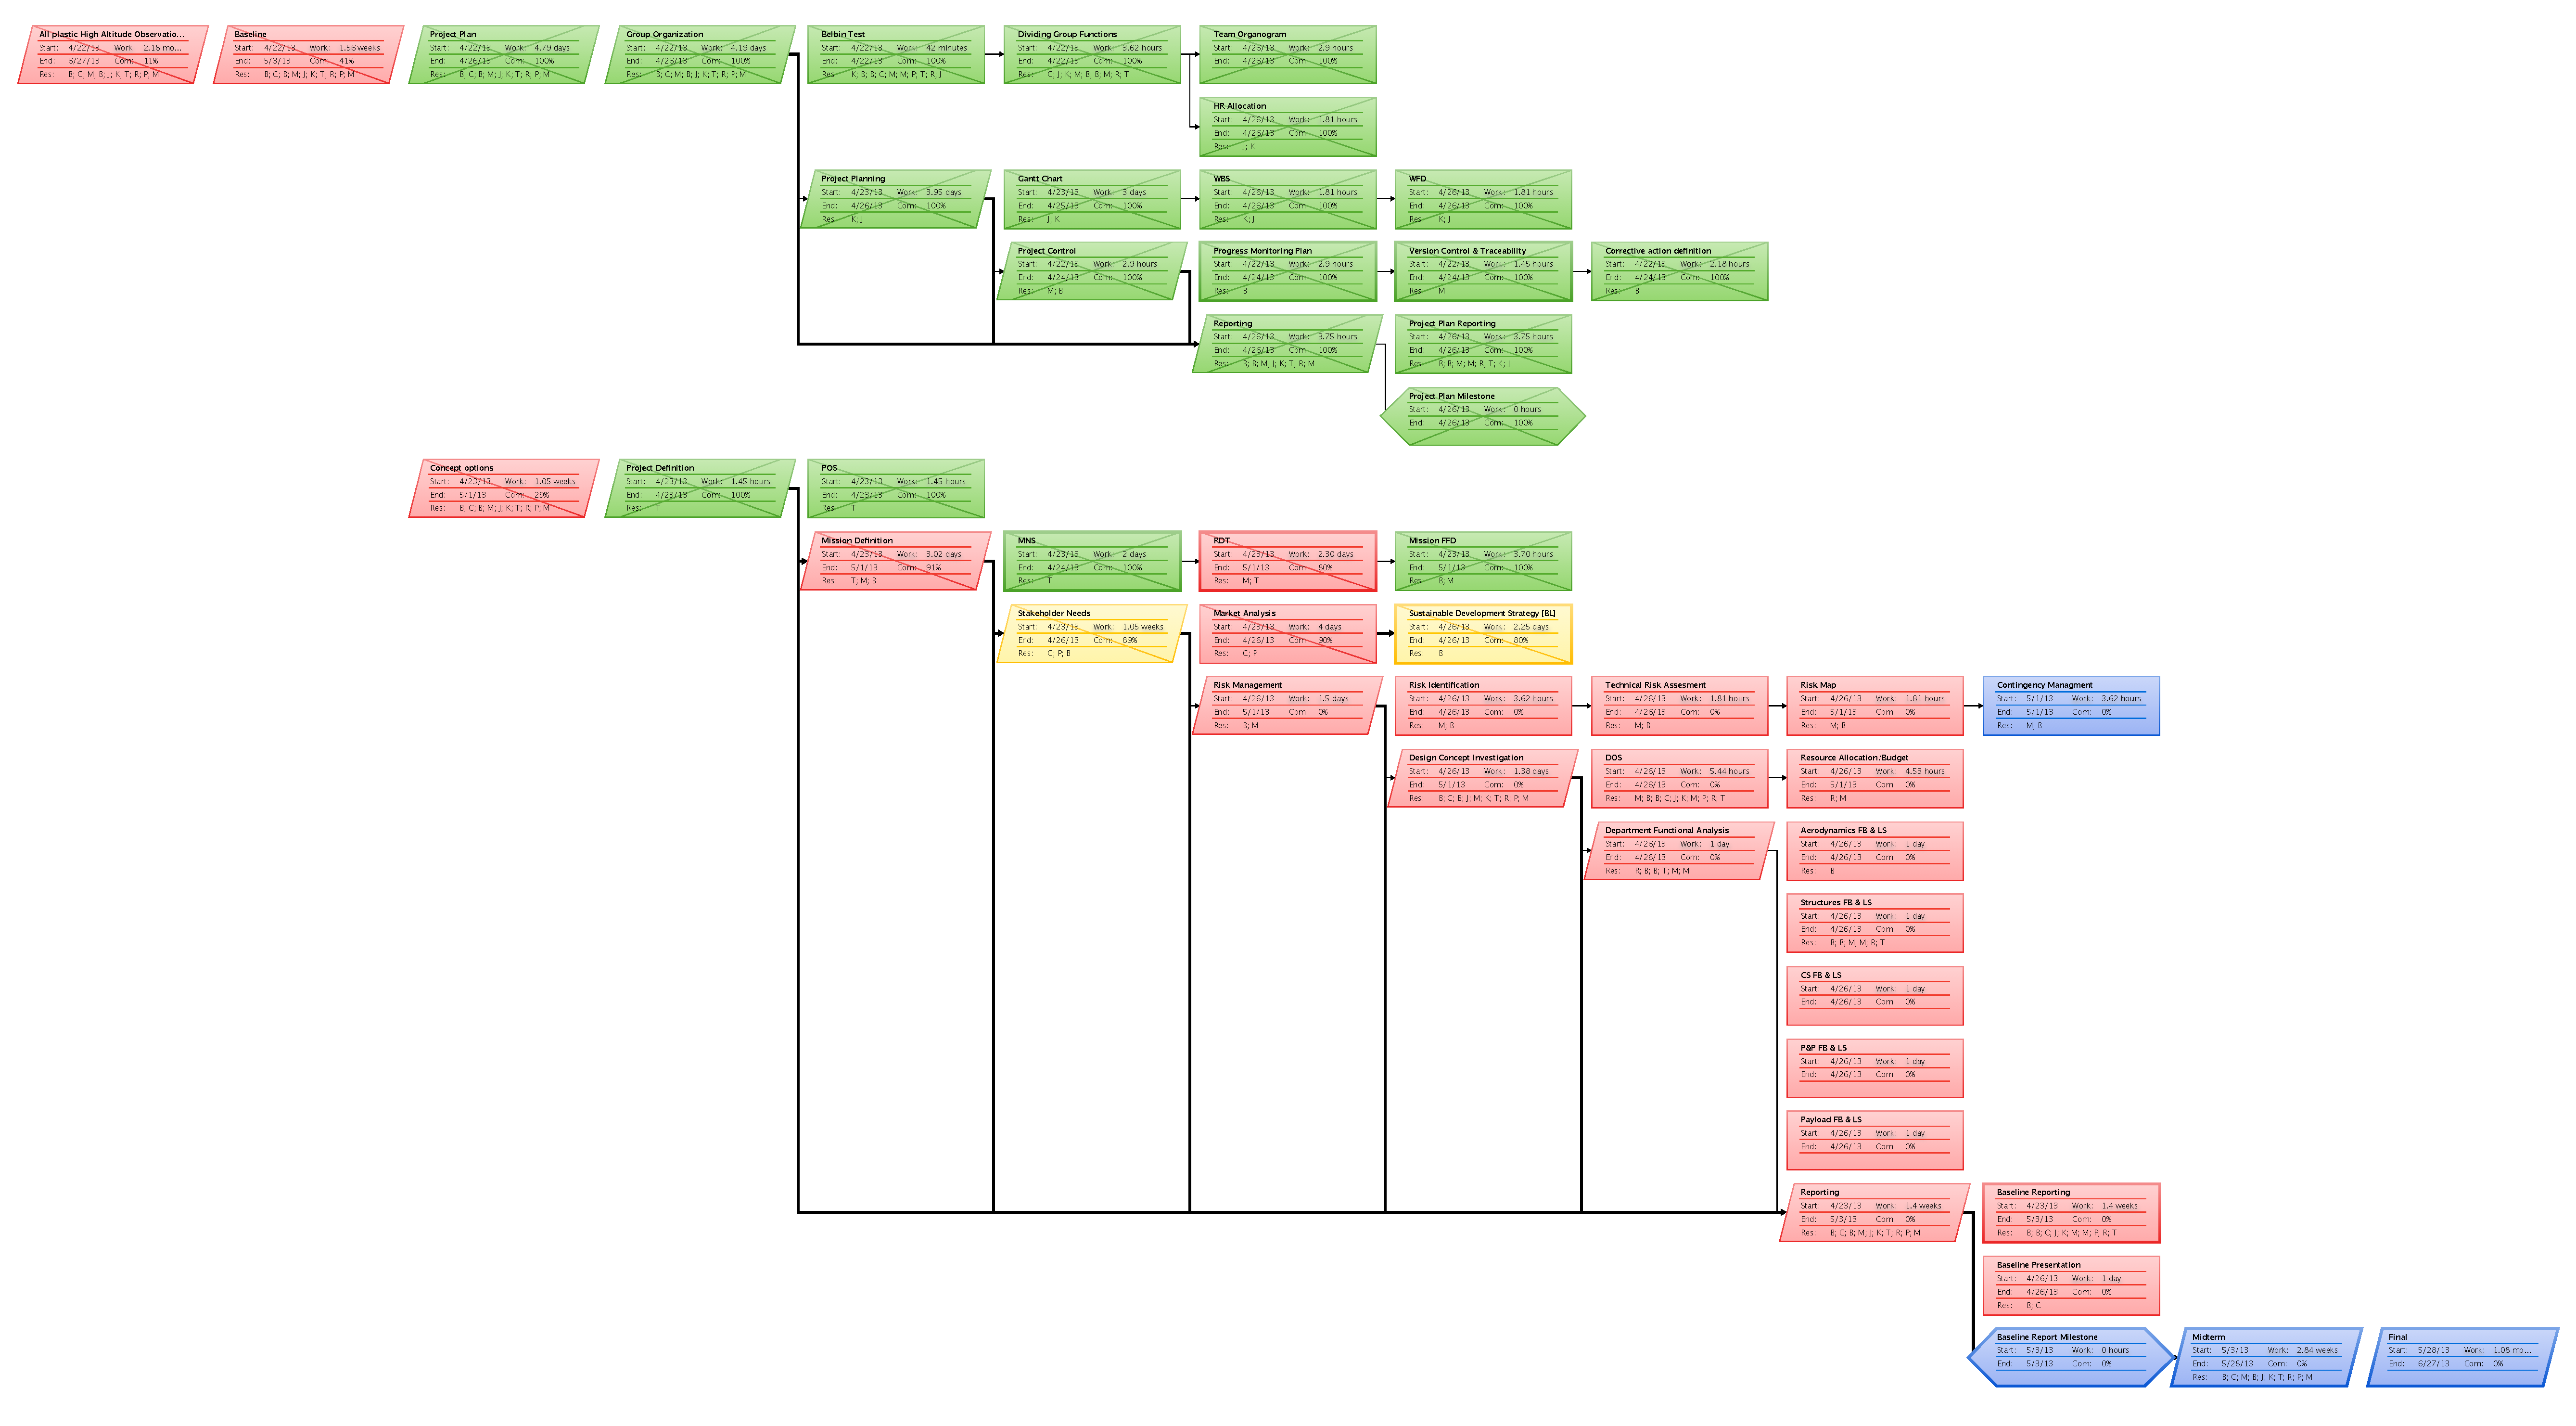
\includegraphics[width=\textheight, angle=270]{Figures/BASEWFD.pdf}
	\caption{WFD of the BR development}
	\label{fig:wfdbr}
	
\end{figure}
\subsection{Midterm Review}
During the midterm part of the project, five concepts will be chosen to further develop and evaluate. Once some predetermined data for these concepts is known, a trade-off can be performed to chose one final concept for further development. The Gantt chart for the Midterm review can be seen in \autoref{fig:ganttmtr}. 

\begin{figure}[H]
	\centering
	
	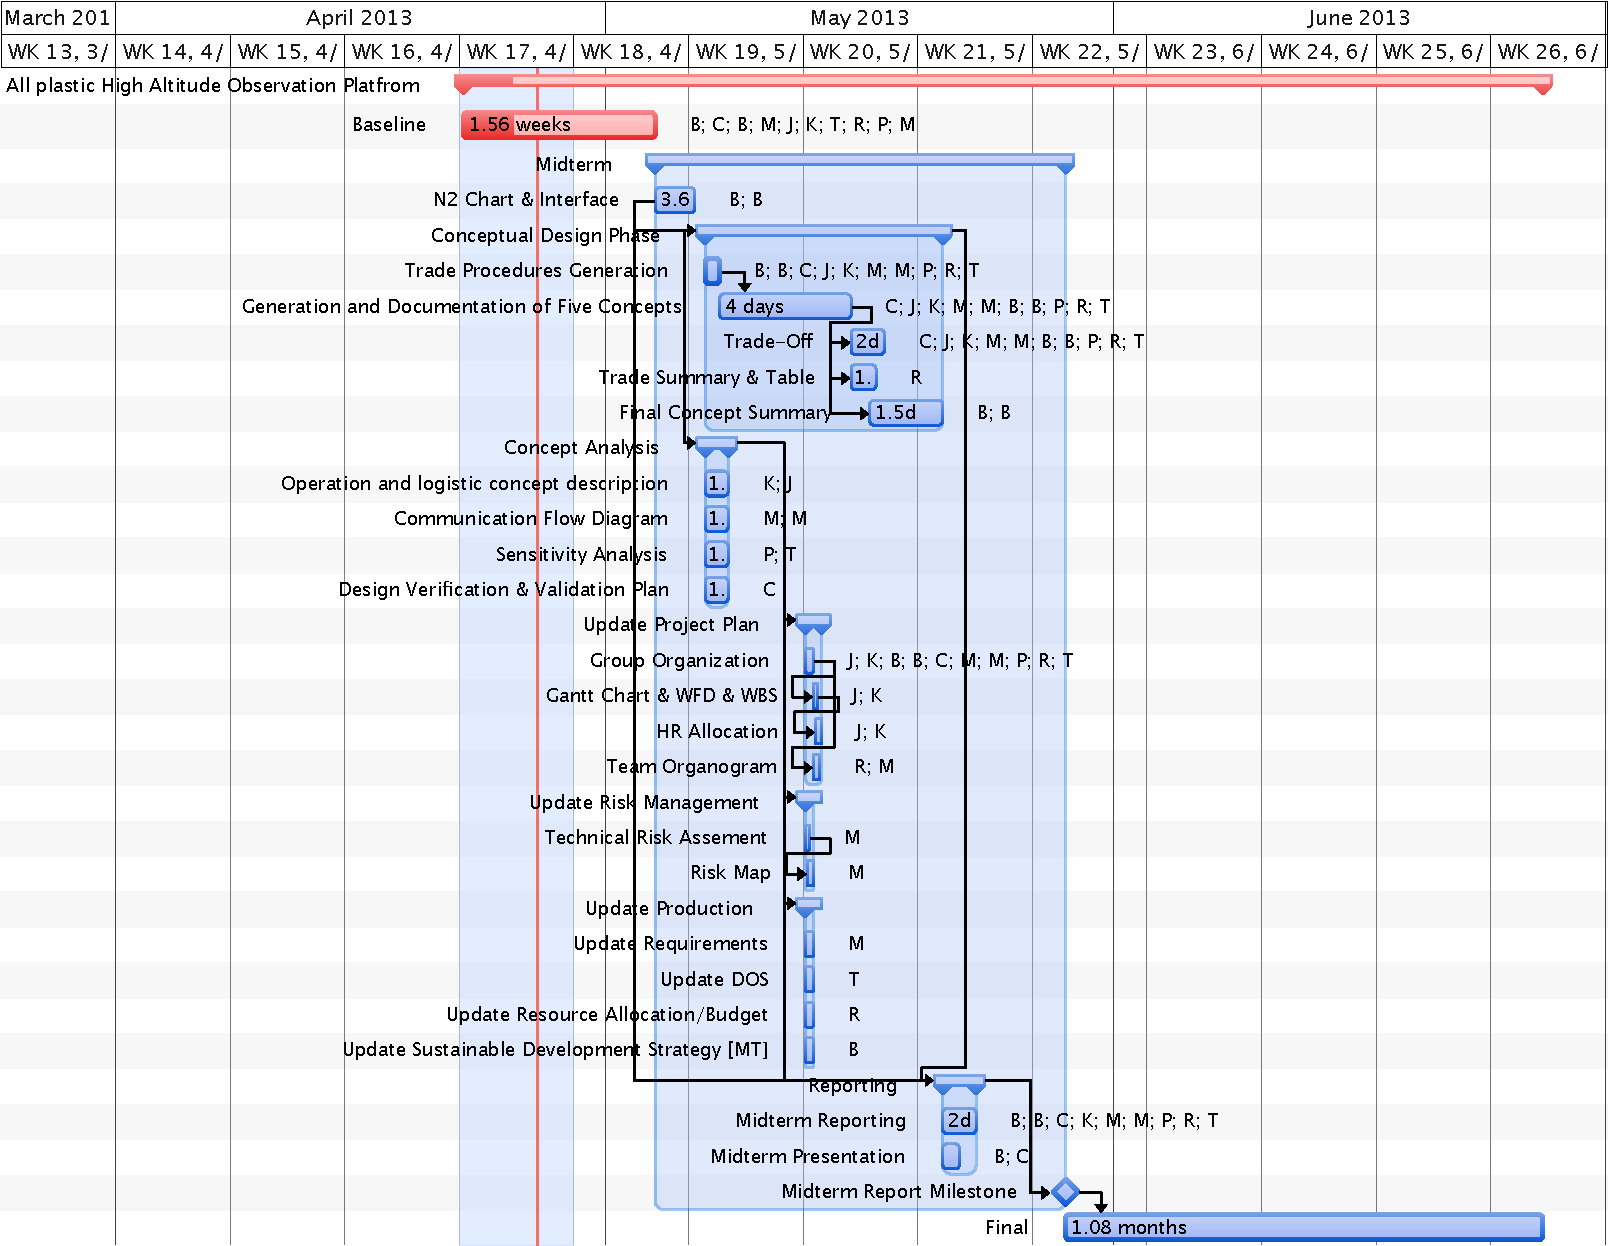
\includegraphics[width=\textwidth]{Figures/MIDGANTT.PDF}
	\caption{Gantt-chart for the development of the MTR}
	\label{fig:ganttmtr}
	
\end{figure}

First the entire group will agree on a trade method rationale and trade criteria. Then the group is split in five groups of two, which each develop a promising concept and generate some data for the previous set criteria. Once this is done, the group comes back together and chooses a final concept. Some analysis is subsequently performed on this concept, such as an operation and logistic investigation and a sensitivity analysis. Finally, a number of documents such as the risk assessment and Gantt chart will be updated at the end of this phase. The entire work-flow logic can be seen in \autoref{fig:wfdmtr}. 
\begin{figure}[H]
	\centering
	
	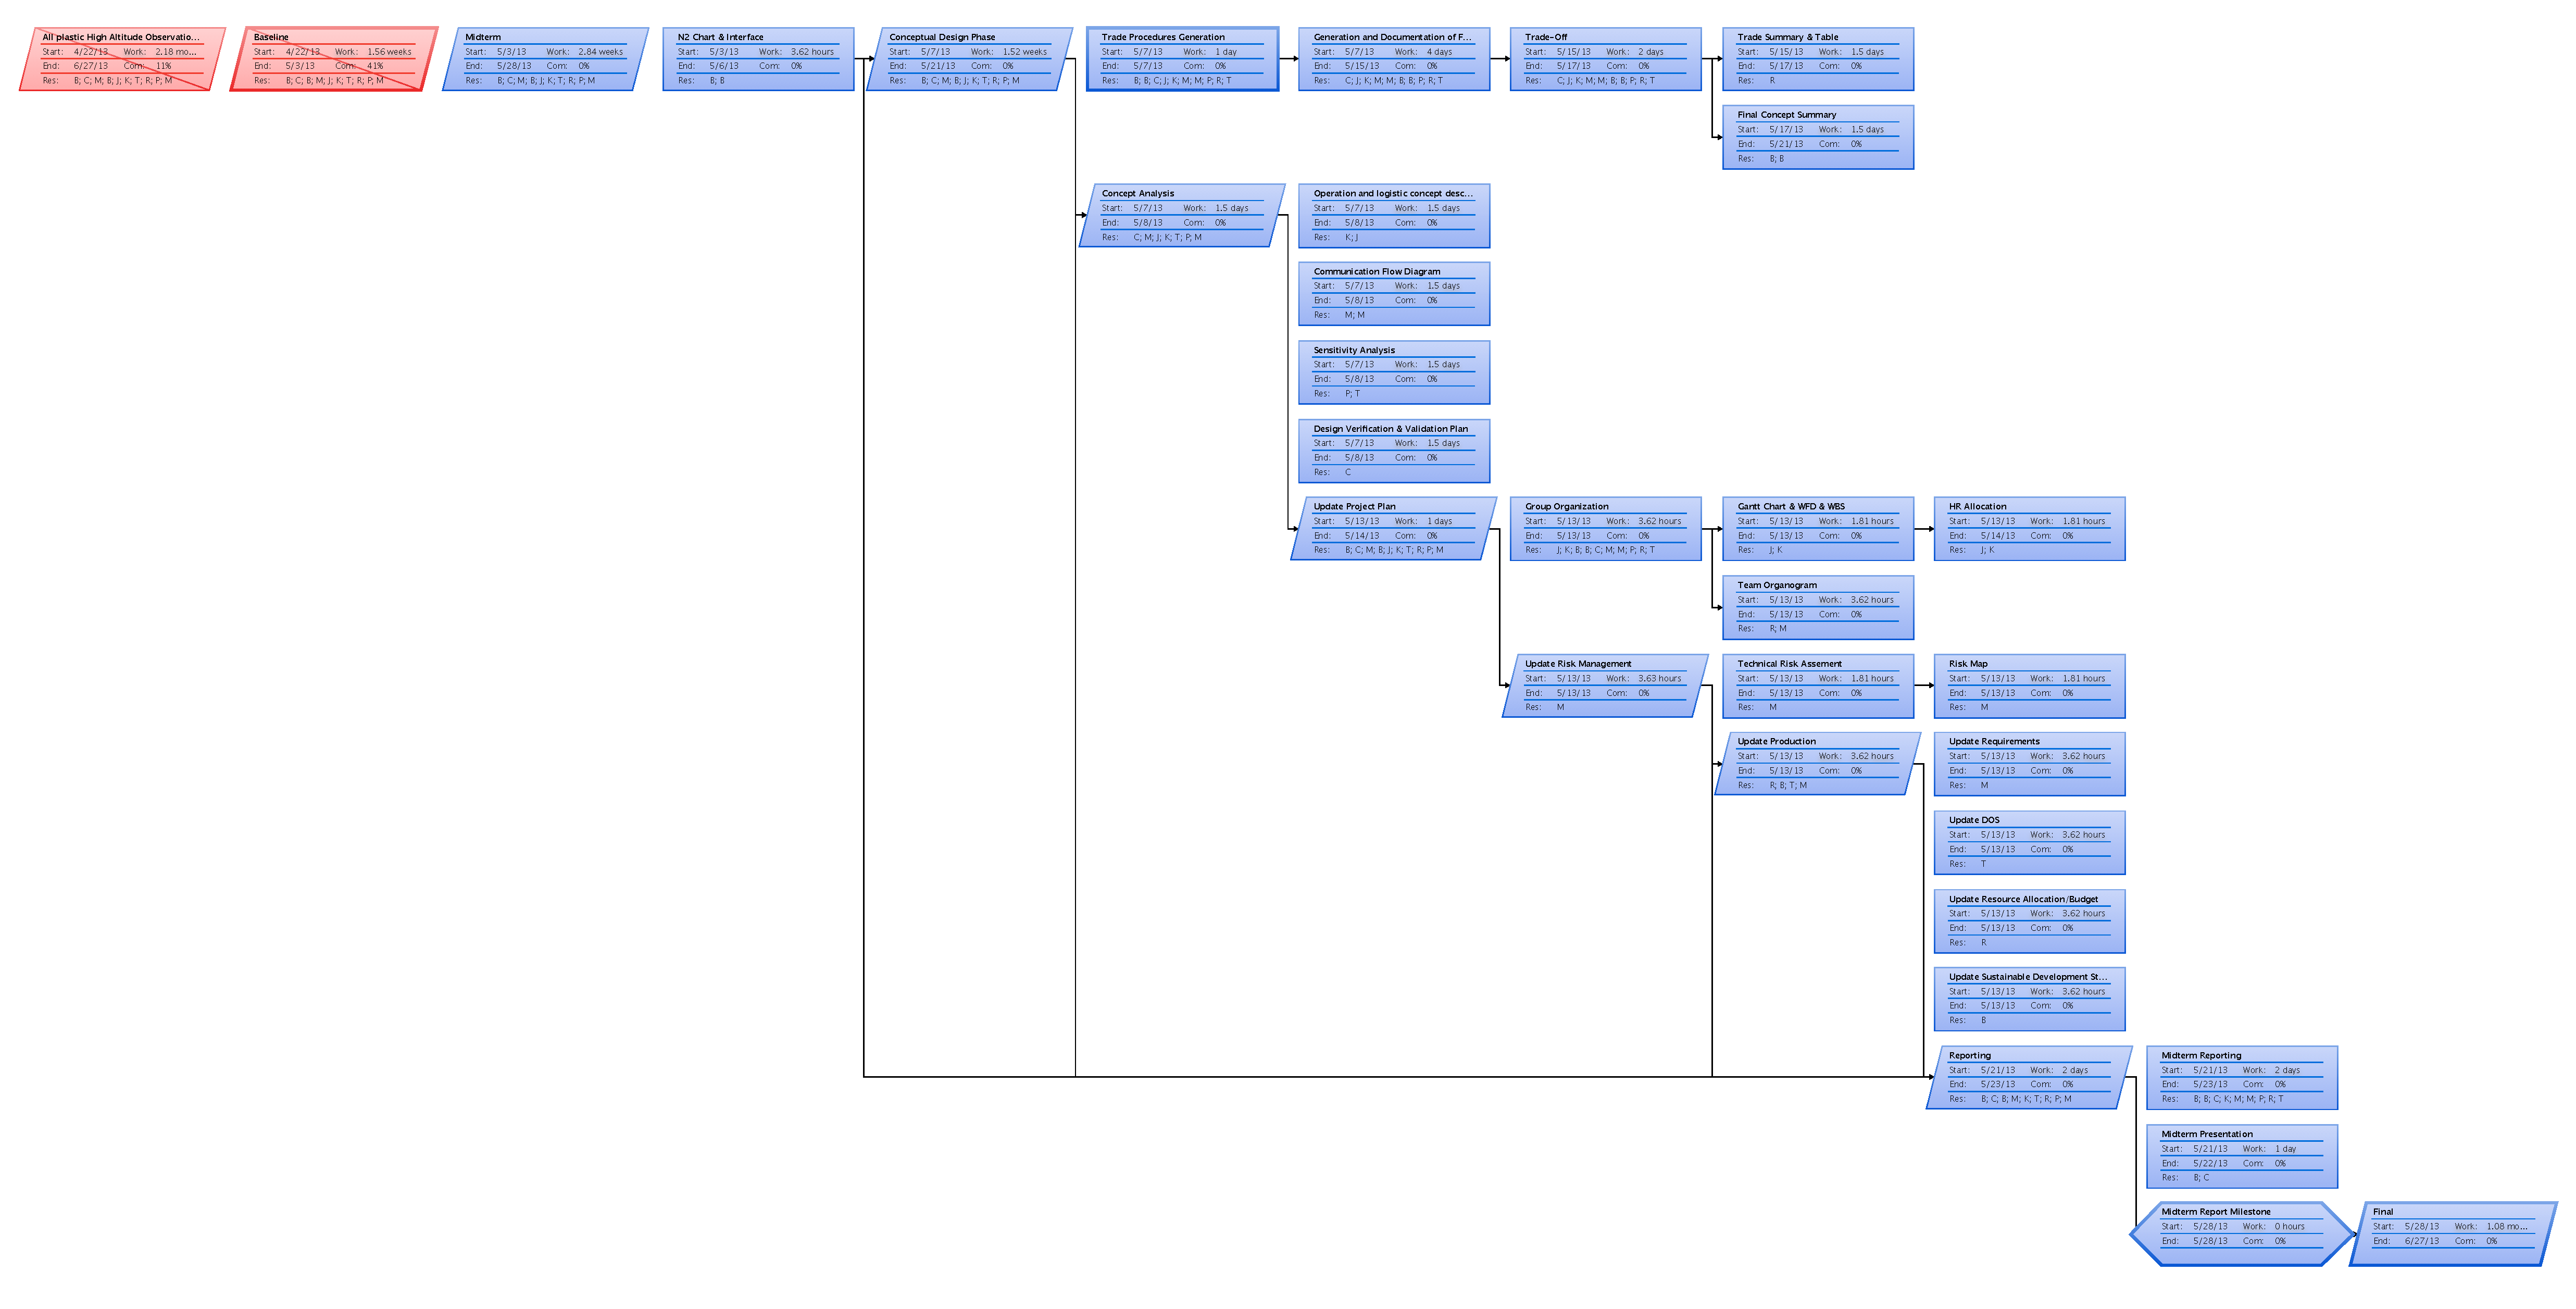
\includegraphics[width=\textheight, angle=270]{Figures/MIDWFD.pdf}
	\caption{WFD of the MTR development}
	\label{fig:wfdmtr}
	
\end{figure}

\subsection{Final Review}
A Gantt chart and Work-Flow Diagram were also created for the Final Review. The schedule is very uncertain for this part of the project, therefore no further elaboration is given here. The charts can be seen in \autoref{fig:ganttfr} and \autoref{fig:wfdfr}.
\begin{figure}[h]
	\centering
	
	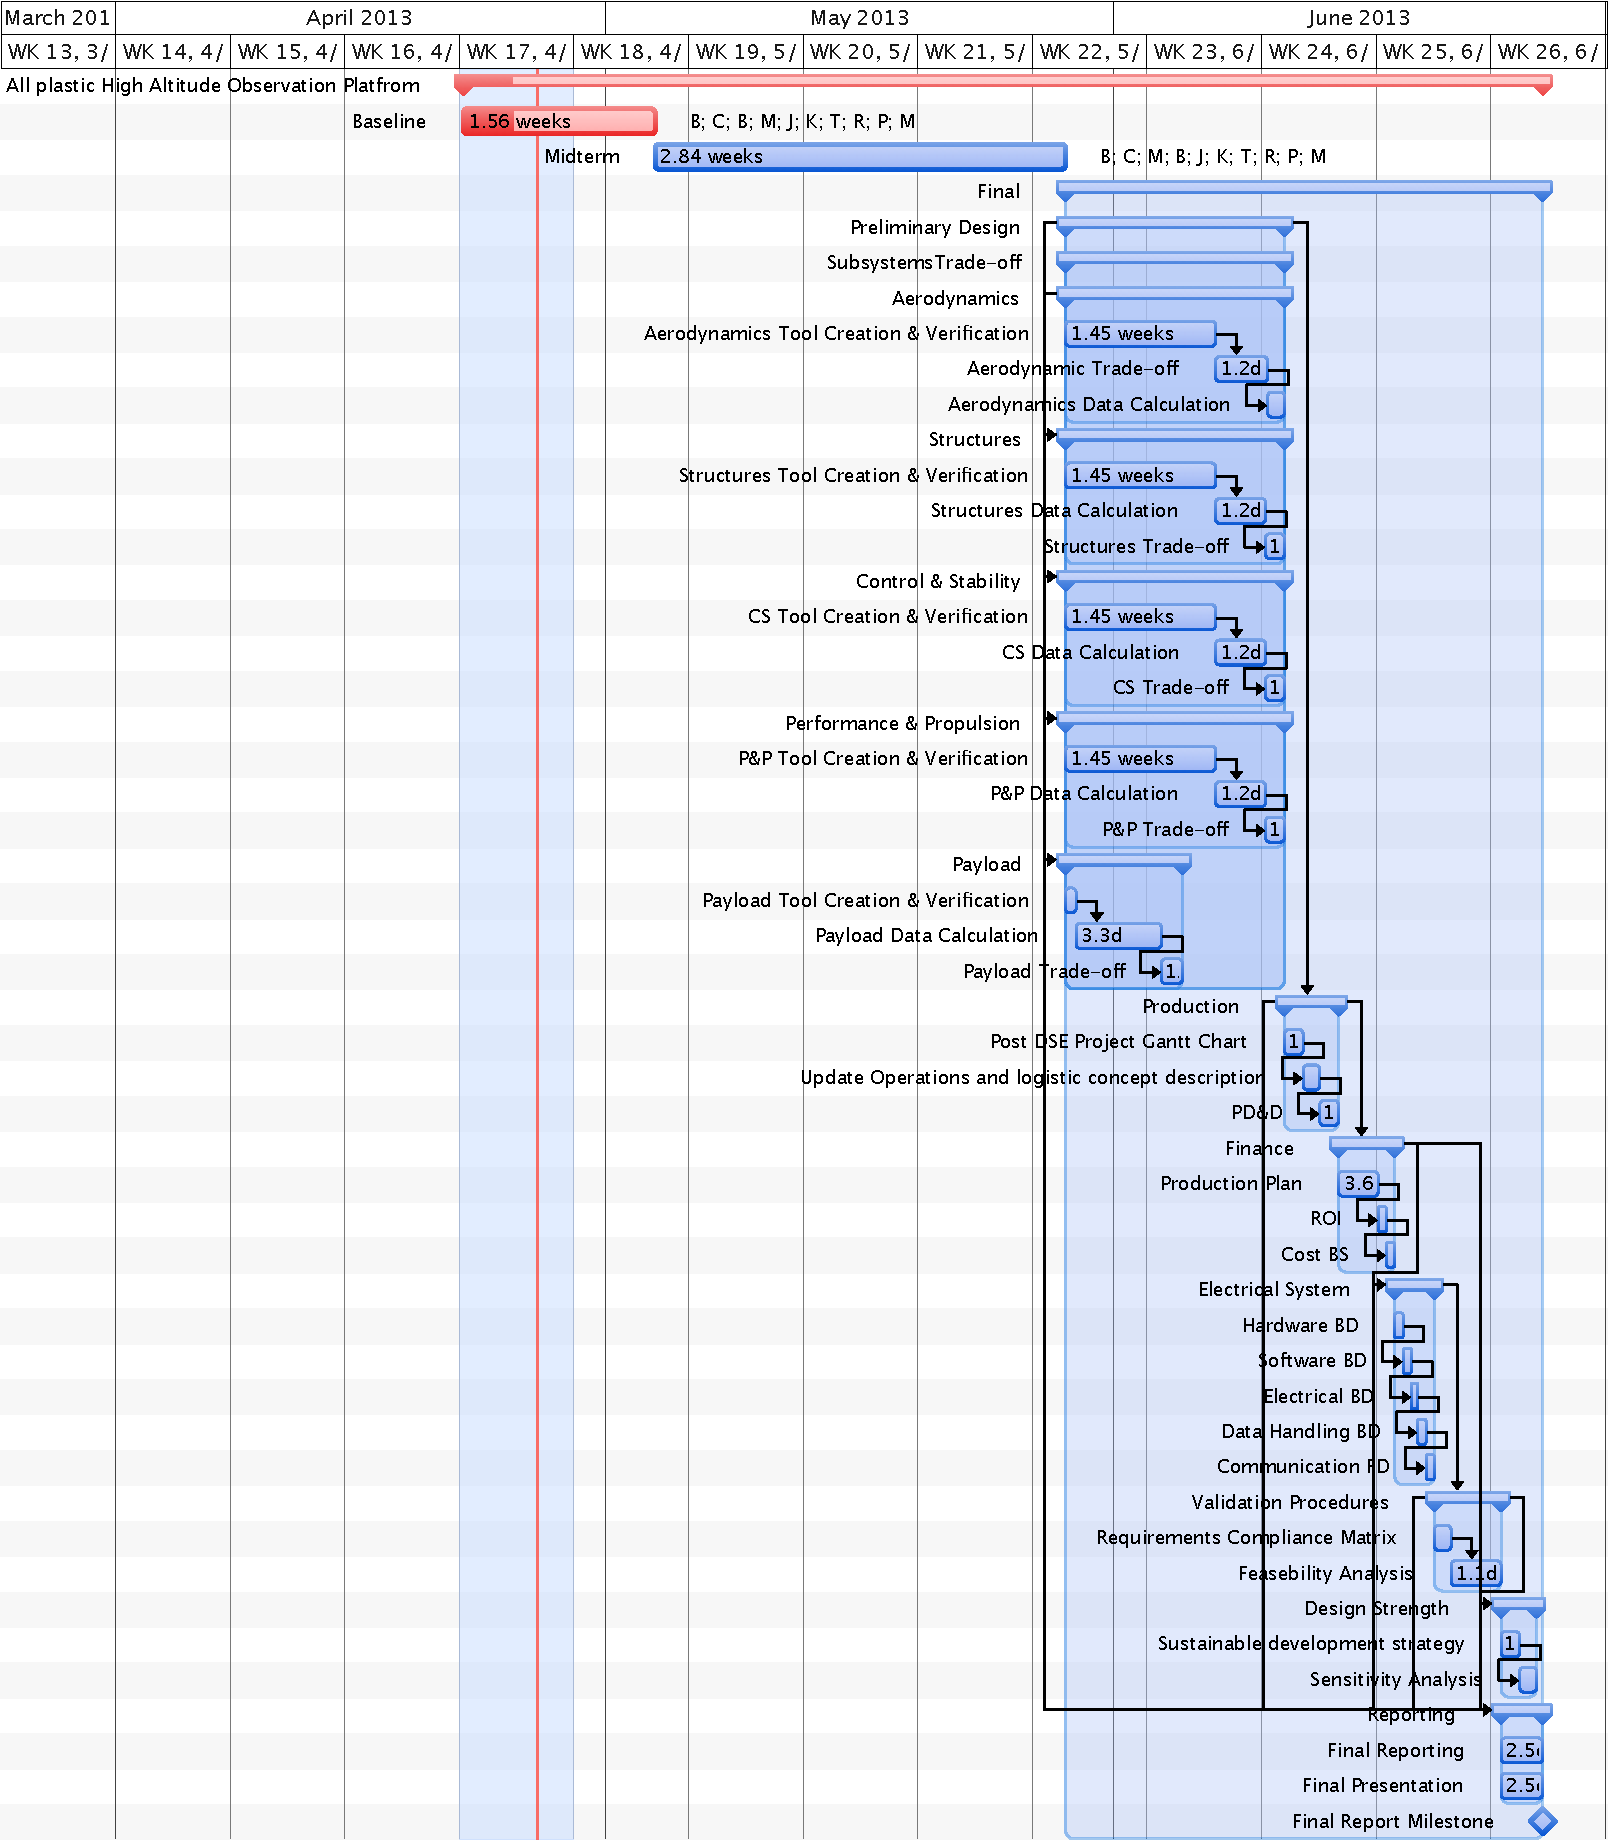
\includegraphics[width=0.8\textwidth]{Figures/FINALGANTT.pdf}
	\caption{Gantt Chart for the Final Review of the FR development}
	\label{fig:ganttfr}
	
\end{figure}
\begin{figure}[H]
	\centering
	
	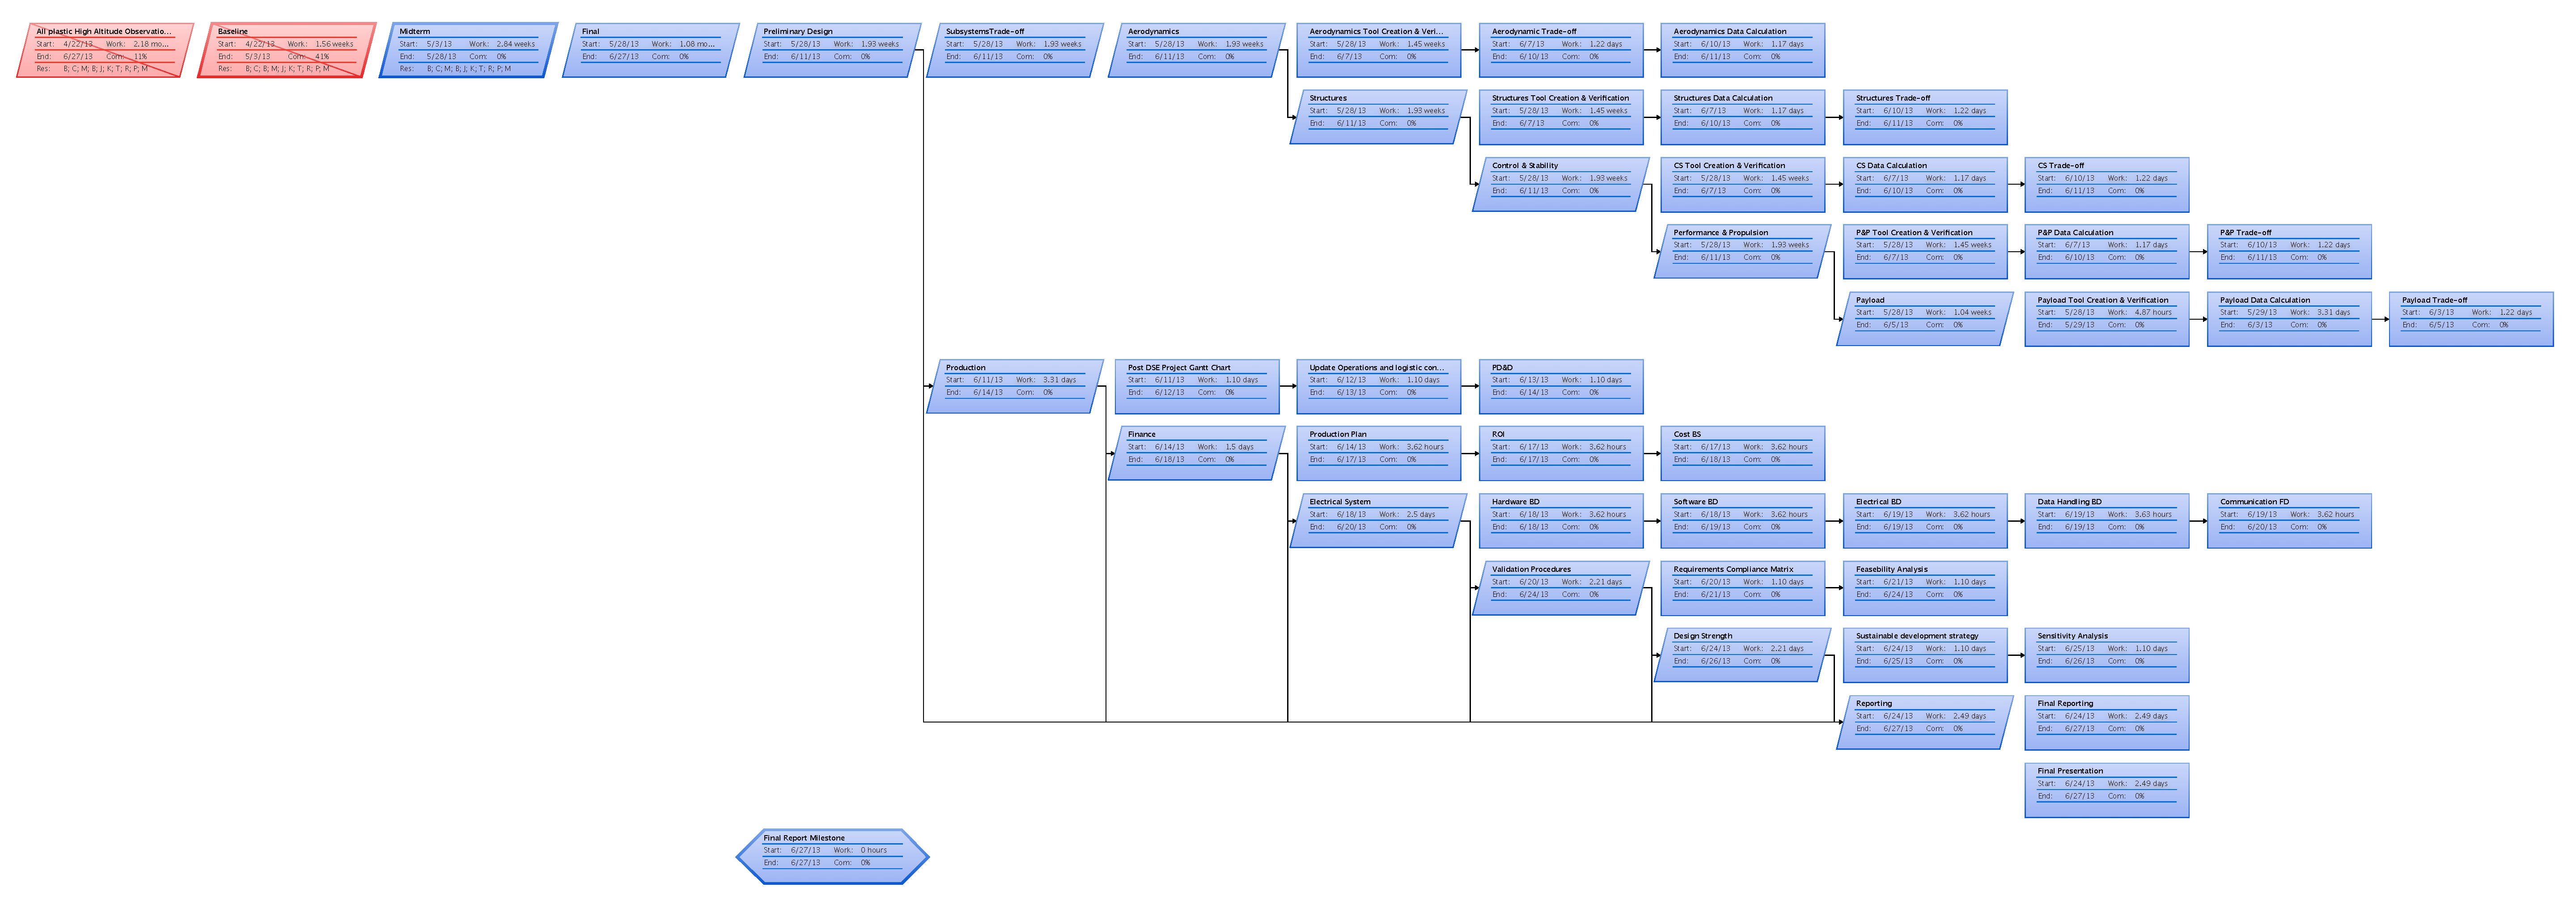
\includegraphics[width=\textheight, angle=270]{Figures/FINALWFD.pdf}
	\caption{WFD of the FR development}
	\label{fig:wfdfr}
	
\end{figure}

\section{Work Breakdown Structure}
The Work Breakdown Structure presents the structure of the entire project in a hierarchical tree and can be seen in \autoref{fig:wbs}. The data for this structure was taken from the Gantt chart. Final review is included in the structure, however little is certain about this part of project and it can be expected this part will change in the future.  

\begin{figure}[H]
	\centering
	
	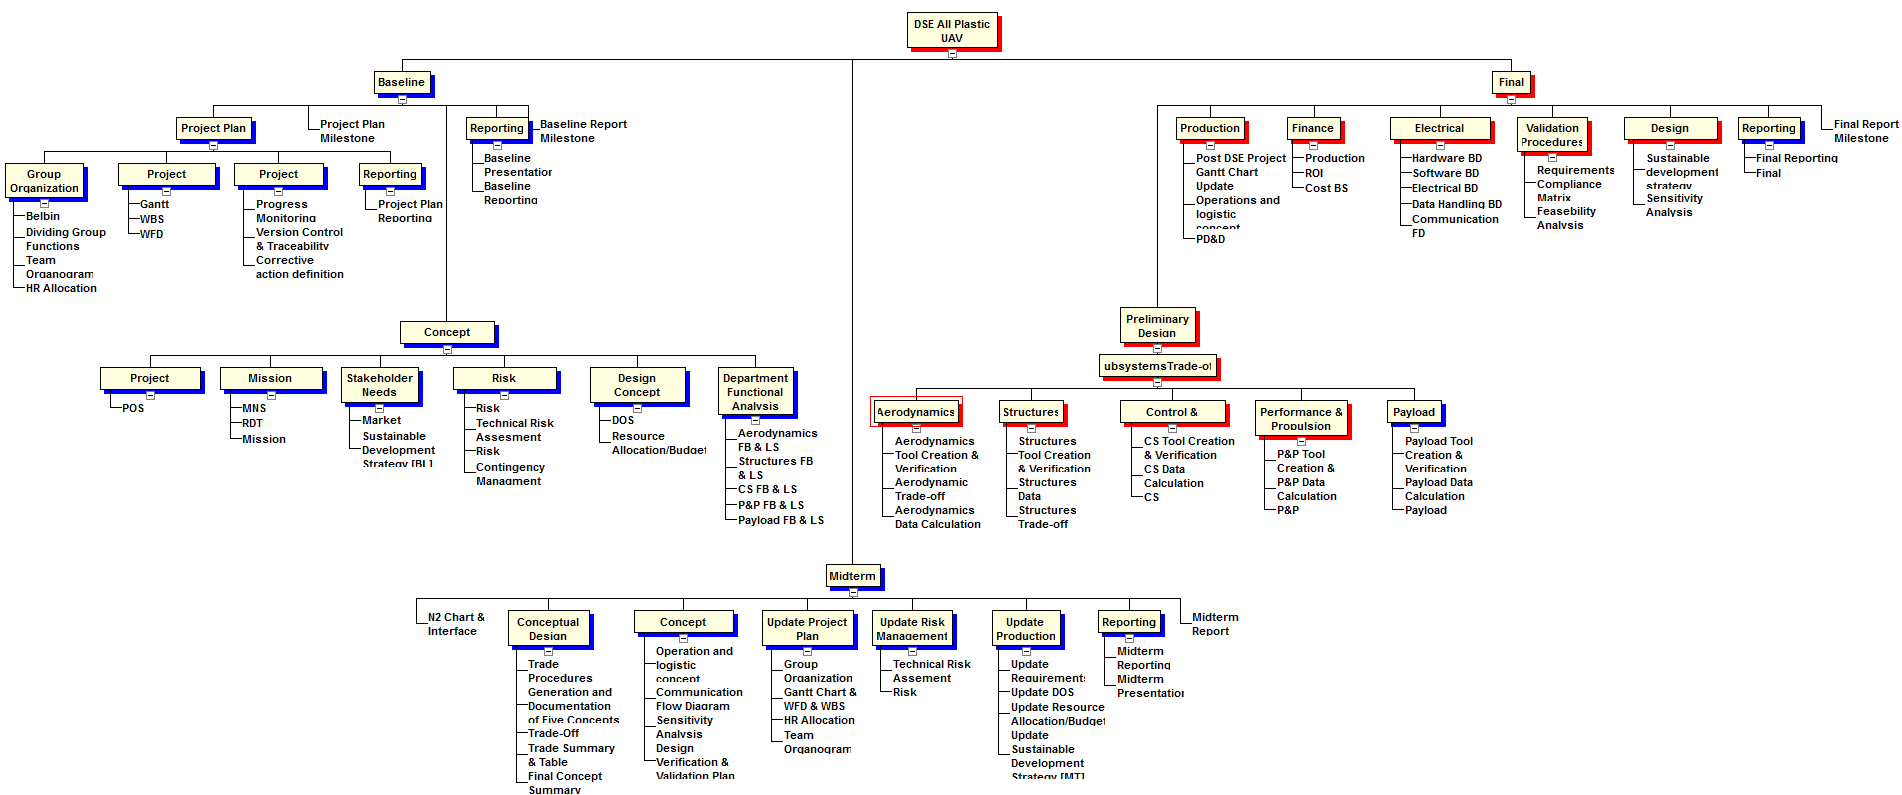
\includegraphics[width=0.8\textheight, angle=270]{Figures/WBS.png}
	\caption{WBS of the entire project}
	\label{fig:wbs}
	
\end{figure}
\section{Schedule Risk}
This sub-chapter will briefly discuss the risk associated with the schedule up to the Midterm Review. The risk associated with planning for the Final Review will not be discussed, since it is too far into the future and little is known about it at this stage of the project. Thus any discussion regarding associated risk will be meaningless. 
\subsection{Baseline Milestone Risk}
When looking at the schedule for the Baseline Review, it can be seen there is no room for slack planned in at all. Even worse, the presentation is actually scheduled to be completed after the milestone. This is possible because the presentation is not part of the report, but of the review which has a slightly later deadline. 
\newline
Zero slack is a big risk. If any critical task is delayed, the milestone will not be met. It is a highly undesirable situation, but cannot be avoided at this point in time due to short period up to the deadline. The consequence is the planning needs to be vigilantly guarded. When it is not met, extra work has to be put in to ensure schedule compliance.
\subsection{Midterm Milestone Risk}
Unlike the Baseline Milestone, the schedule for the Midterm milestone contains considerable slack. Since this is a design phase, it can be expected tasks will take longer than anticipated. This was also emphasized during a discussion with one of the coaches. 
\newline
The risk for delay to the Midterm Milestone is difficult to quantify at this stage. It is estimated it will be lower compared to the Baseline Report Risk. 

\end{document}